% \documentclass[article]{standalone}
\documentclass[tikz]{standalone}

\usepackage{hyperref}
% \usepackage{hyperref, tikz}

% Determine flow chart stuff
\usetikzlibrary{shapes.geometric, arrows} % Arrows library
% Define block styles
%\tikzstyle{decision} = [diamond, draw, fill=blue!20, text width=4.5em, text badly centered, node distance=3cm, inner sep=0pt]
\tikzstyle{bblock} = [rectangle, draw, fill=blue!20, text width=11em, text centered, rounded corners, minimum height=4em, node distance = 7em]
\tikzstyle{yblock} = [rectangle, draw, fill=yellow!20, text width=11em, text centered, rounded corners, minimum height=4em, node distance = 7em]
\tikzstyle{rblock} = [rectangle, draw, fill=red!20, text width=11em, text centered, rounded corners, minimum height=4em, node distance = 7em]
\tikzstyle{wblock} = [rectangle, draw, fill=white, text width=11em, text centered, rounded corners, minimum height=4em, node distance = 7em]
\tikzstyle{secret} = [text width=1em, text centered, rounded corners, minimum height=1em, node distance = 2em]
\tikzstyle{line} = [draw, very thick, color=black, -latex']
\tikzstyle{rcloud} = [draw, ellipse, fill=red!20, text width=10em, node distance=5cm, minimum height=4em]
\tikzstyle{wcloud} = [draw, ellipse, fill=white, text width=10em, node distance=5cm, minimum height=4em]

%Change to sans serif font
\renewcommand{\familydefault}{\sfdefault}		%Alone with use Computer Modern sans serif
\usepackage{sansmathfonts}

\hypersetup{
    linktoc=all,     %set to all if you want both sections and subsections linked
}

\begin{document}

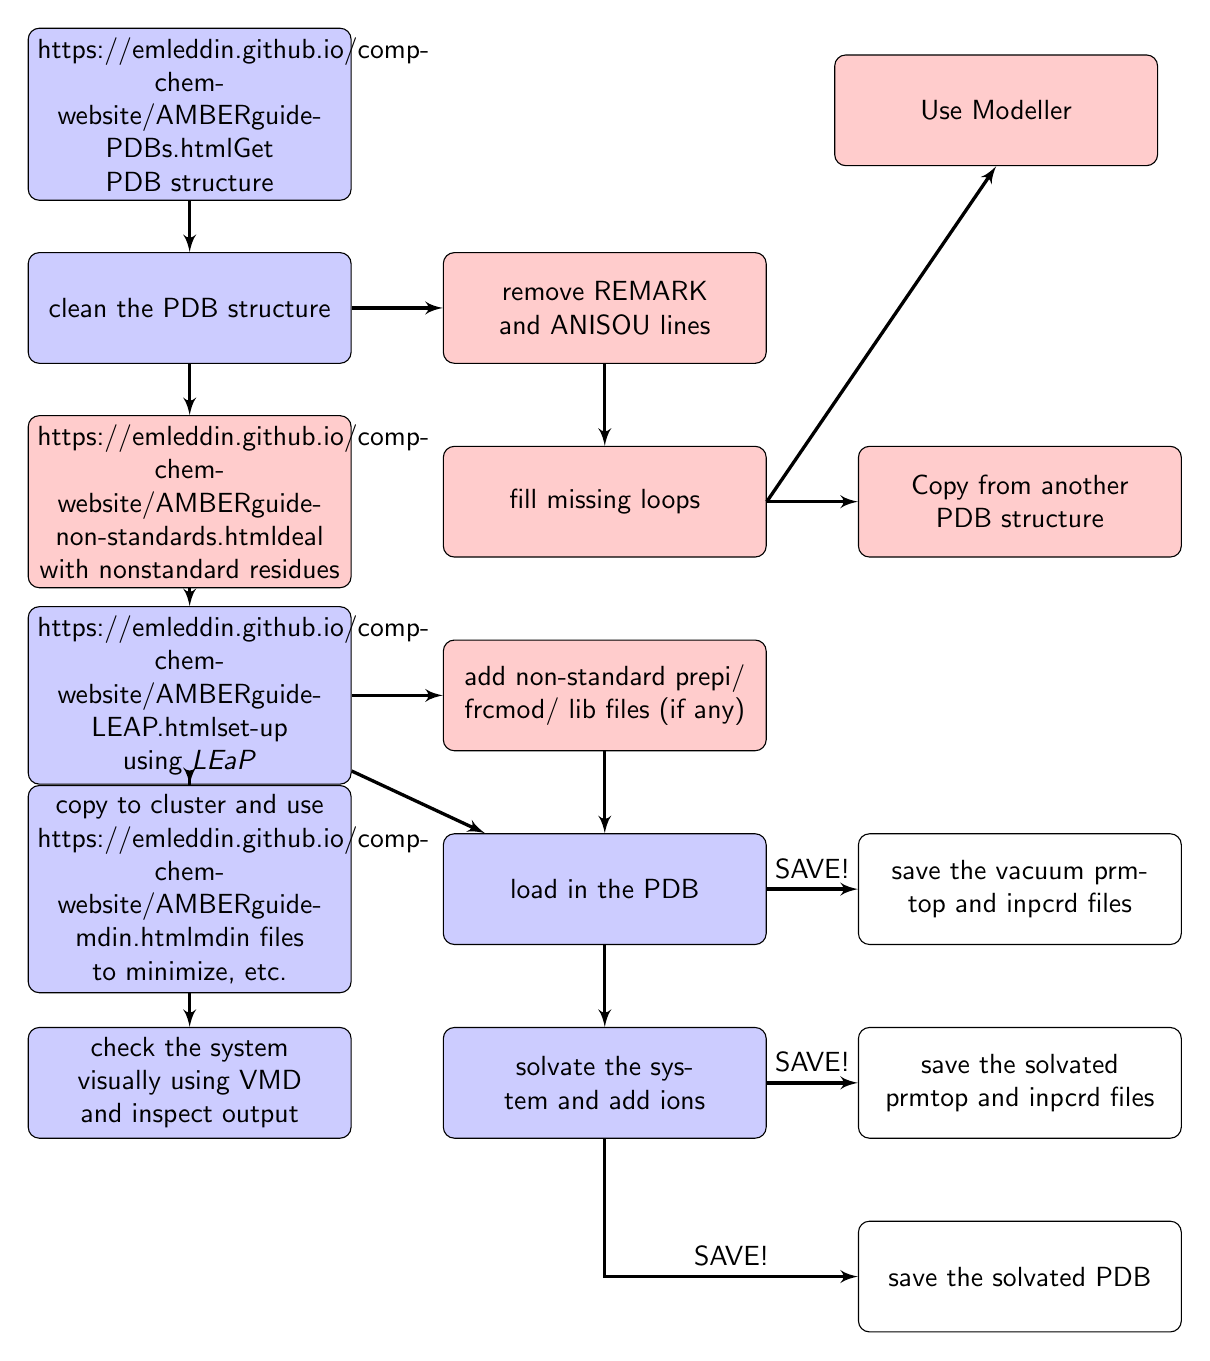
\begin{tikzpicture}[node distance = 0.5cm, auto]
    % Place nodes
    \node [bblock] (pdb) {\href{https://emleddin.github.io/comp-chem-website/AMBERguide-PDBs.html}{Get PDB structure}};
%    \node [bblock] (pdb) {\href{AMBERguide-PDBs.html}{Get PDB structure}};
    \node [bblock, below of=pdb] (clean) {clean the PDB structure};
    \node [rblock, right of=clean, node distance=15em] (remove) {remove REMARK and ANISOU lines};
    \node [rblock, below of=remove] (loops) {fill missing loops};
    \node [rblock, above right of=loops, node distance=20em] (model1) {Use Modeller};
    \node [rblock, right of=loops, node distance=15em] (model2) {Copy from another PDB structure};
    \node [rblock, below of=clean] (nonstand) {\href{https://emleddin.github.io/comp-chem-website/AMBERguide-non-standards.html}{deal with nonstandard residues}};
    \node [bblock, below of=nonstand] (AMBER) {\href{https://emleddin.github.io/comp-chem-website/AMBERguide-LEAP.html}{set-up using \emph{LEaP}}};
%    \node [rblock, below of=clean] (nonstand) {\href{AMBERguide-non-standards.html}{deal with nonstandard residues}};
%    \node [bblock, below of=nonstand] (AMBER) {\href{AMBERguide-LEAP.html}{set-up using \emph{LEaP}}};
    \node [rblock, right of=AMBER, node distance=15em] (addnon) {add non-standard prepi/ frcmod/ lib files (if any)};
    \node [bblock, below of=addnon] (loadpdb) {load in the PDB};
    \node [wblock, right of=loadpdb, node distance=15em] (save1) {save the vacuum prmtop and inpcrd files};
    \node [bblock, below of=loadpdb] (solvate) {solvate the system and add ions};
    \node [wblock, right of=solvate, node distance=15em] (save2) {save the solvated prmtop and inpcrd files};
    \node [wblock, below of=save2] (save3) {save the solvated PDB};
    \node [bblock, below of=AMBER] (cruntch) {copy to cluster and use \href{https://emleddin.github.io/comp-chem-website/AMBERguide-mdin.html}{mdin} files to minimize, etc.};
%    \node [bblock, below of=AMBER] (cruntch) {copy to cluster and use \href{/AMBERguide-mdin.html}{mdin} files to minimize, etc.};
    \node [bblock, below of=cruntch] (check) {check the system visually using VMD and inspect output};
    % Draw edges
    \path [line] (pdb) -- (clean);
    \path [line] (clean.east) -- (remove);
    \path [line] (remove) -- (loops);
    \path [line] (loops.east) -- (model1.south);
    \path [line] (loops.east) -- (model2);
    \path [line] (clean) -- (nonstand);
    \path [line] (nonstand) -- (AMBER);
    \path [line] (AMBER.east) -- (addnon);
    \path [line] (AMBER) -- (loadpdb);
    \path [line] (addnon) -- (loadpdb);
    \path [line] (loadpdb.east) -- node {SAVE!} (save1);
    \path [line] (loadpdb) -- (solvate);
    \path [line] (solvate.east) -- node {SAVE!} (save2);
    \path [line] (solvate) |- node [near end] {SAVE!}  (save3);
    \path [line] (AMBER) -- (cruntch);
    \path [line] (cruntch) -- (check);
    %\path [line] (loops) -| node [near start] {yes} (update);
    %\path [line] (update) |- (identify);
    %\path [line] (decide) -- node {no}(stop);
    %\path [line,dashed] (expert) -- (init);
    %\path [line,dashed] (system) -- (init);
    %\path [line,dashed] (system) |- (evaluate);
\end{tikzpicture}

\end{document}
